%\clearpage
\def\delequal{\mathrel{\ensurestackMath{\stackon[1pt]{=}{\scriptstyle\Delta}}}}
%//==============================--@--==============================//%
\subsection*{\underline{2.1} Circuito RL Série}
%//==============================--A--==============================//%
\subsubsection*{(a) Obtenha o regime transitório relativo à corrente $i$ para $t \ge 0$.}
\label{subsubsec_a}
\paragraph{Resposta:}
Por aplicação direta da Lei de Indução, $\overrightarrow{\nabla} \times \overrightarrow{E} = -\dfrac{\partial}{\partial t}\overrightarrow{B}$, é facilmente derivada a EDO linear de primeiro grau que rege o sistema. Naturalmente, como o gerador não impõe nenhuma tensão para $t < 0$, verifica-se o seguinte par:

$$
    \begin{cases}
        u_g(t) = i(t)R + L \dfrac{di(t)}{dt} \\
        i(0^-) = i(0^+) = 0
    \end{cases}
$$

Deste modo, procura-se a solução homogénea (\textit{natural}), $i_n(t)$, e a solução particular (\textit{forçada}), $i_f(t)$, tal que a resposta do PVI se verifique pela justaposição das soluções mencionadas, i.e.:

\begin{equation}
    \label{eq1}
    i(t) = i_n(t) + i_f(t)
\end{equation}

\noindent
\underline{Solução natural:} 

A equação linear homogénea $L \dfrac{di(t)}{dt} + i(t)R = 0$, tem como equação característica: 

$$
    Ls + R = 0 \iff s = -\frac{R}{L} \implies \tau = -\frac{1}{s} = \frac{L}{R} = \frac{1}{3000} = 0.(3)\ \text{ms} 
$$
$$
    \therefore i_n(t) = I_n e^{-t/\tau}\ \text{A}
$$

\vspace{0.5cm}
\noindent
\underline{Solução forçada:}
\vspace{0.25cm}

No domínio dos fasores é trivialmente deduzida a resposta forçada. Atendendo à equação que rege o circuito no domínio do tempo, observa-se:

$$
    \bar{U}_g = R \bar{I}_f + j\omega L \bar{I}_f = \bar{Z}_{eq} \bar{I}_f \implies \bar{I}_f = \frac{\bar{U}_g}{\bar{Z}_{eq}} = \frac{U_g}{Z_{eq}}e^{j(\alpha - \measuredangle \bar{Z}_{eq})}
$$

$$
\implies i_f(t) = \frac{U_g}{Z_{eq}} \cos{(\omega t + \alpha - \measuredangle \bar{Z}_{eq})} = I_f \cos{(\omega t + \alpha - \varphi)}
$$

$$
    \begin{cases}
        I_f = U_g/\sqrt{R^2+(\omega L)^2} \approx 0.634 \sqrt{2}\ \text{mA} \\
        \varphi = \measuredangle \bar{Z}_{eq} = \arctan{(\dfrac{\omega L}{R})} \approx 1.476\ \text{rad}
    \end{cases}
$$

$$
    \therefore i_f(t) \approx 0.634 \sqrt{2}\cdot \cos{(\omega t - 3.046)}\ \text{mA}\text{, para $\alpha = -\pi/2$.}
$$

\clearpage
Com especial atenção ao enunciado em \hyperref[eq1]{(1)} e às condições iniciais do PVI, procede-se à determinação do valor inicial do regime \textit{natural} para que se obtenha a solução geral da equação diferencial (i.e., $i(t)$).

$$
    i(0) = 0 \iff i_n(0) = -i_f(0) \implies I_n = -0.634\sqrt{2}\cdot \cos{(-3.046)} \cdot 10^{-3}
$$

$$
    \implies I_n \approx 0.893\ \text{mA}
$$

$$
    \therefore i(t) = 0.634\sqrt{2}\cdot [\ \cos{(\omega t - 3.046)} - \cos{(3.046)}\cdot e^{-3000t}\ ]\ \text{mA}
$$
\hfill \ensuremath{\Box}
%//==============================--B--==============================//%
\subsubsection*{(b) Determine a expressão que permite calcular aproximadamente os instantes em que a corrente $i$ tem extremos, supondo que estes extremos se dão quando $\cos{(\omega t + \alpha - \varphi)} = \pm 1$, e
determine também a expressão que permite determinar o valor desses extremos para
$\alpha = -\pi/2$.}
\label{subsubsec_b}
\paragraph{Resposta:}
Tomando a aproximação enunciada, encontramos os extremos quando a expressão $\cos{(\omega t_x + \alpha - \varphi)} = \pm 1$ se verifica. Deste modo, é uma reação imediata\footnotemark concluir que:

$$
    \omega t_x + \alpha -\varphi = k\pi\text{,}\ \forall k \in \mathbb{Z}_{0}^{+}
$$

Assim, os instantes $t_x$ correspondentes aos e\textbf{x}tremos (para $\alpha = -\pi/2$) são:

$$
    \implies t_x = \frac{k\pi - \alpha + \varphi}{\omega} \iff t_x = \frac{k\pi + 3.046}{10000\pi} \approx (100k + 96.957)\ \mu\text{s}\text{,}\ \forall k \in \mathbb{Z} 
$$

Segue-se que a expressão que nos permite calcular os extremos (\textit{aproximadamente}) pode ser descrita por:

$$
    i(t_x) = 0.634\sqrt{2}\cdot [\ (-1)^k - \cos{(3.046)}\cdot e^{-3(100k + 96.957)\cdot 10^{-3}} \ ]\cdot 10^{-3} \iff
$$
$$
\iff i(t_x) = 0.897\cdot (-1)^k + 0.893\cdot e^{-3(100k + 96.957)\cdot 10^{-3}}\ \text{mA}\text{,}\ \forall k \in \mathbb{Z}_{0}^{+}
$$
\hfill \ensuremath{\Box}

\footnotetext{Note-se que $t \ge 0$, pelo que $k$ \textit{não pode} ser um inteiro negativo!}
%//==============================--C--==============================//%
\clearpage
\subsubsection*{(c) Utilizando a expressão da alínea anterior determine os cinco primeiros extremos, no caso de $\alpha = -\pi/2$. Para o primeiro extremo determine a solução exata, através de um processo
numérico. Verifique que a raiz exata é, neste caso, bastante próxima do valor aproximado.}
\label{subsubsec_c}
\paragraph{Resposta:}
Utilizando os resultados da alínea a que a atual sucede, encontram-se sinteticamente na \hyperref[tab1]{Tab. 1} os valores \textit{aproximados} para as abcissas dos extremos, bem como os seus valores (para $\alpha = -\pi/2$).

\begin{table}[ht]
    \centering
    \caption{Primeiros cinco extremos determinados, e as suas abcissas respetivas.}
    \label{tab1}
    \begin{tabular}{SSS}
        \toprule
        $k$ & $t_x/\mu\text{s}$ & $i(t_x)/\text{mA}$ \\ \midrule
        0  & 96.957 & 1.565  \\
        1  & 196.957 & -0.402 \\
        2  & 296.957 & 1.263 \\
        3  & 396.957 & -0.626 \\
        4  &  496.957 & 1.098 \\ \bottomrule
    \end{tabular}
\end{table}
\hfill \ensuremath{\Box}

Em seguida, utiliza-se o \underline{método de Newton-Rhapson} de modo a comparar o valor \textit{aproximado} obtido anteriormente para $k=0$ com a solução exata.
$$
    \frac{di(t)}{dt} = 0.634\sqrt{2}\cdot [\ -\omega\sin{(\omega t - 3.046)} + 3000\cos{(3.046)}\cdot e^{-3000t}\ ] = 0
$$

A expressão anterior é naturalmente referente ao cálculo dos extremos de $i(t)$, deste modo temos que:
$$
    f(x) = 0 \implies f(x) = \frac{di(x)}{dx} = 0.634\sqrt{2}\cdot [\ -\omega\sin{(\omega x - 3.046)} + 3000\cos{(3.046)}\cdot e^{-3000x}\ ]
$$
$$
    \implies f'(x) = \frac{d^2i(x)}{dx^2} = 0.634\sqrt{2}\cdot [\ -\omega^2\cos{(\omega x - 3.046)} - 9\cdot 10^{6}\cos{(3.046)}\cdot e^{-3000x}\ ]
$$

O \underline{método de Newton-Rhapson} visa obter, no nosso caso, de uma forma mais refinada, a abcissa do primeiro extremo calculado. Este é um método \textit{iterativo} que termina com a restrição imposta no enunciado: $\left\vert x_{n+1} - x_n\right\vert < 10^{-6}$.
\begin{equation}
    x_{n+1} = x_n - \frac{f(x_n)}{f'(x_n)}   
\end{equation}

Seja $x_0 = t_x(k=0) = 96.957\ \mu\text{s}$, aplicando o método mencionado, obtem-se:
$$
    x_{1} = x_{0} - \frac{f(x_0)}{f'(x_0)} \implies x_{1} \approx 94.680\ \mu\text{s} \implies \left\vert x_{1} - x_0\right\vert \approx 2.277 \cdot 10^{-6} > 10^{-6}
$$

Note-se que é necessária uma segunda iteração, para melhor refinar a abcissa:
$$
    x_{2} = x_{1} - \frac{f(x_1)}{f'(x_1)} \implies x_{2} \approx 94.678\ \mu\text{s} \implies \left\vert x_{2} - x_1\right\vert \approx 2.371 \cdot 10^{-9} < 10^{-6}
$$

Chegando à condição de paragem, conclúi-se que $x_2$ é uma boa aproximação da raiz exata. Verifica-se que a \textit{aproximação} está, de facto, relativamente próxima a este novo resultado:
$$
    \text{Erro}(\%) = \left\vert\frac{t_x(k=0)-x_2}{x_2}\right\vert \cdot 100 = \left\vert\frac{96.957-94.678}{94.678}\right\vert \cdot 100 \approx 2.41 \% 
$$

Assim, o valor da solução exata, obtido através do processo \textit{iterativo}, é para este extremo:
$$
    i(x_2) = 0.634\sqrt{2}\cdot [\ \cos{(\omega x_2 - 3.046)} - \cos{(3.046)}\cdot e^{-3000x_2}\ ] \approx 1.566\ \text{mA}
$$

Comparando com o valor obtido através da aproximação:
$$
    \text{Erro}(\%) = \left\vert\frac{i(t_x(k=0))-i(x_2)}{i(x_2)}\right\vert \cdot 100 \approx 0.073 \%
$$

Como esperado, também se encontra bastante próximo.

\hfill \ensuremath{\Box}

\vspace{0.75cm}

\iffalse
\begin{figure}[!h]  
    \centering
        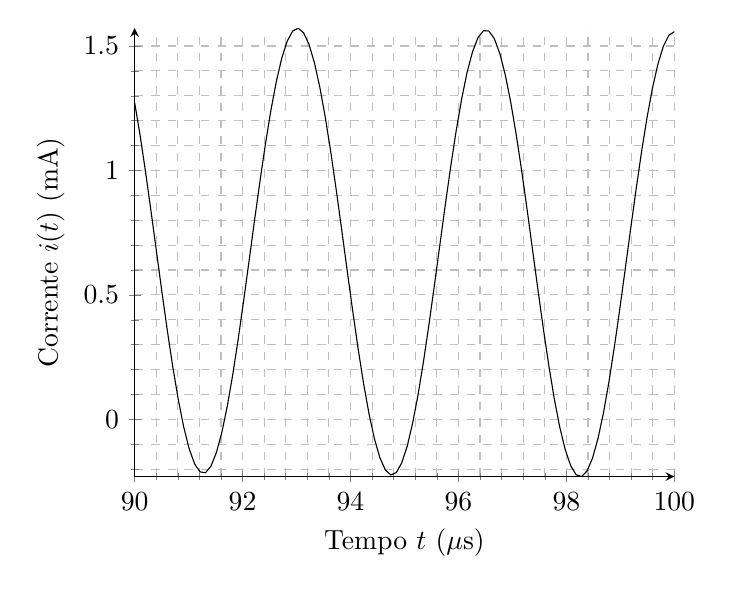
\begin{tikzpicture}
            \begin{axis}[
                axis lines = left,
                xlabel = {Tempo $t$ ($\mu$s)},
                ylabel = {Corrente $i(t)$ (mA)},
                grid style=dashed,
                grid=both,
                minor tick num=4
            ]

            \addplot[
                domain=90:100, 
                samples=100, 
                color=black
            ]
            {0.896*cos(deg(1.8*x-180)) + 0.893*e^(-0.003*x)};
            
            %\addplot [only marks,mark=*,dashed,color=darkgray] coordinates { (\fnum,2*pi*1.8/sqrt(2)};
            %\node[label={160:{\color{darkgray} $(f_{n1},\frac{Q_0}{\sqrt{2}})$}},inner sep=2pt] at (0.956757,7.997189) {};
            
            %\addplot [only marks,mark=*,dashed,color=darkgray] coordinates { (\fndois,2*pi*1.8/sqrt(2)};
            %\node[label={55:{\color{darkgray} $(f_{n2},\frac{Q_0}{\sqrt{2}})$}},inner sep=2pt] at (1.045186,7.997189) {};
            
            %\addplot +[mark=none,color=darkgray,dashed] coordinates {(\fnum, 0.5) (\fnum, 2*pi*1.8)};
            
            %\addplot +[mark=none,color=darkgray,dashed] coordinates {(\fndois, 0.5) (\fndois, 2*pi*1.8)};
            
            %\addlegendentry{}
            \end{axis}
        \end{tikzpicture}
\caption{Proximidade entre os valores aproximados e os valores obtidos através do processo \textit{iterativo}.} \label{fig:proximidade} 
\end{figure}
\fi
%//==============================--D--==============================//%
\clearpage
\subsubsection*{(d) Considere agora que se desliga o gerador quando a tensão vai a passar por zero de valores negativos para positivos, supondo que o circuito está em regime forçado. Determine a solução para $i(t)$, calculando o valor inicial da corrente $I_0$ e a constante de tempo $\tau$.}
\label{subsubsec_d}
\paragraph{Resposta:}
Naturalmente, como consequência imediata da remoção da tensão do gerador, verifica-se que a solução do regime forçado é nula, i.e., $i_f(t) \equiv 0$, $\forall t$.

Com a aplicação da Lei de Indução verifica-se uma equação diferencial \text{homogénea} tal como esperado:
$$
    \overrightarrow{\nabla} \times \overrightarrow{E} = -\dfrac{\partial}{\partial t}\overrightarrow{B} \implies L \dfrac{di(t)}{dt} + i(t)R = 0
$$

A forma da solução desta equação já é conhecida de \hyperref[subsubsec_b]{\underline{2.1} (b)}; é para além disto adiantado que a constante de tempo $\tau$ se mantém inalterada (como seria de esperar), seja $\tau = 0.(3)$ ms.

Para a nova situação, verifica-se a solução geral:
$$
    i(t) = i_n(t) = I_0\cdot e^{-t/\tau}\ \text{A}
$$

Sequencialmente, para determinar $I_0$ é necessário determinar os instantes em que o gerador passa por zero de valores negativos para positivos:
$$
    u_g(t_0) = U_g \cos{(\omega t + \alpha)}\text{, e como $\alpha = -\pi/2$} \implies u_g(t) = U_g \sin{(\omega t)}\ \text{V}
$$

Por conseguinte, $t_0$ é um ponto da forma: $t_0 = 2k\pi/\omega$, $\forall k \in \mathbb{Z}$. 


Até ao instante $t_0$, o circuito funciona em regime forçado, e assim, devido à continuidade de $i(t)$ que nos é assegurada, faz-se uso da equação da corrente forçada, estabelecida na alínea \hyperref[subsubsec_b]{\underline{2.1} (b)}, para calcular a amplitude neste dado instante.

Visto que não ocorrem saltos energéticos infinitos, voltamos ao resultado bastante familiar:
$$
    i(t_0^-) = i(t_0^+) = I_0 \iff I_0 = 0.634 \sqrt{2}\cdot \cos{(\omega t_0 - 3.046)}
$$

$$
    \implies I_0 = 0.634 \sqrt{2}\cdot \cos{(2k\pi-3.046)} \approx -0.893\ \text{mA, }\forall k \in \mathbb{Z}
$$
Em suma, a solução para $i(t)$ é: 
$$
    \therefore i(t) = I_0\cdot e^{-t/\tau} \approx -0.893\cdot e^{-3000t}\ \text{mA}\text{, }\forall t \ge t_0
$$
\hfill \ensuremath{\Box}
%//==============================--E--==============================//%
\subsubsection*{(e) Verifique que para $t = \tau$ se tem: \\ $$i(\tau) = \dfrac{I_0}{e}$$}
\label{subsubsec_e}
\paragraph{Resposta:} Trivialmente verificado por substituição direta na expressão deduzida na alínea anterior:

$$
    i(t) = I_0\cdot e^{-t/\tau} \implies i(\tau) = I_0\cdot e^{-\tau/\tau} = I_0\cdot e^{-1} = \frac{I_0}{e}\ \text{A}
$$
\hfill \ensuremath{\Box}
%//==============================--@--==============================//%